\documentclass[a4paper, 12pt]{article}
\usepackage[english, russian]{babel}
\usepackage{listings}
\usepackage[top=2cm, bottom=2cm, left=2cm, right=2cm, bindingoffset=0pt]{geometry}
\usepackage{hyperref}
\usepackage{amsmath,amsfonts,amssymb,amsthm,mathtools}
\usepackage[T2A]{fontenc}
\usepackage[utf8]{inputenc}
\newtheorem*{theorem*}{Теорема}
\theoremstyle{definition}
\newtheorem*{definition*}{Определение}
\theoremstyle{definition}
\newtheorem*{example*}{Пример}
\renewcommand\qedsymbol{$\blacksquare$}
\usepackage{tikz}
\usetikzlibrary{positioning}
\usetikzlibrary {graphs}
\usepackage{graphicx}
\graphicspath{ {./images/} }

\renewcommand{\leq}{\leqslant}
\renewcommand{\geq}{\geqslant}

\title{Типы уравнений}
\author{Бирюк Илья Александрович}

\begin{document}
  \maketitle
  \newpage
  \tableofcontents
  \newpage
  %\chapter{Основные понятия, связанные с термином "граф"}
  \section{Определение простого графа}
  Пусть $V\neq\varnothing$ - конечное множество и $V^{(2)}$ - множество
  всех двухэлементных подмножеств $V$. $(V^{(2)}=\{U\subseteq V||U|=2\})$.
  Упорядоченная пара $(V,E)$, где $E\subseteq V^{(2)}$ называется \textbf{простым графом}, вершинами которого являются элементы $V$, а рёбрами - элементы $E$.
  \textbf{Пример:}

    $V=\{1,2,3,4,5,6\}, E=\{\{1,5\},\{2,3\},\{1,4\},\{2,4\},\{4,5\},\{3,5\}\}$
    
    \begin{tikzpicture}[main/.style = {draw, circle, thin}]
      \node[main](1){$1$};
      \node[main](2)[below right of=1]{$2$};
      \node[main](6)[below left of=1][anchor=east]{$6$};
      \node[main](5)[below of=6]{$5$};
      \node[main](4)[below right of=5]{$4$};
      \node[main](3)[below right of=2]{$3$};
      \draw[thick] (1) -- (5) -- (4) -- (3) -- (2) -- (4);
      \draw[thick] (5) -- (3);
    \end{tikzpicture}
    
    Число $|V|$ называют \textbf{порядком графа}, а число $|E|$ - \textbf{размером графа}.
    $$G=(V,E), V=V(G), E=E(G)$$

    Если порядок графа равен n, а размер равен m, то говорят, что это \textbf{(n,m)-граф}.

    Две веришины $u$ и $v$ в графе \textbf{смежные}, если $\{u,v\}\in E(G)$. Два ребра $e_1,e_2$ \textbf{смежные}, если $e_1\cap e_2\neq\varnothing$

    Вершина $v$ и ребро $e$ \textbf{инцедентны} если $v\in e$

    \begin{tikzpicture}[main/.style = {draw, circle, thin}]
      \node[main](u){u};
      \node[main](v)[right =1]{v};
      \draw (u) -- node[anchor=south]{e} (v);
    \end{tikzpicture}
    
    Примечание: $\{u,v\}=uv$

    \textbf{Окружением веришины} $u$ в графе $G$ называют множество: $N_G(u)=\{v\in V(G)|uv\in E(G)\}$

    \begin{definition*}
      Число $deg_Gv=|N_G(v)|$ - мощность окружения вершины $v$ - называют \textbf{степенью вершины} в $G$
    \end{definition*}

    Пусть $v\in V(G)$:
    \begin{enumerate}
      \item $deg_Gv=0\leftrightarrow v$ - \textbf{изолированная вершина}
      \item $deg_Gv=|V(G)|-1\leftrightarrow v$ - \textbf{доминирующая вершина}
      \item $deg_Gv=1\leftrightarrow v$ - \textbf{висячая вершина}
    \end{enumerate}

    \begin{definition*}
      Граф $G$ называют \textbf{регулярным}, если он имеет одинаковые степени вершин.
    \end{definition*}
    \begin{definition*}
      Граф $G$ называют \textbf{K-регулярным}, если $\forall v\in V(G),deg(v)=k$.
    \end{definition*}
    \begin{definition*}
      $K_n$ - \textbf{полный граф}(граф со всеми возможными вершинами)
    \end{definition*}
  \section{Некоторые обобщения графов}
  \begin{enumerate}
    \item Мультиграф
    
    \begin{definition*}
      \textbf{Мультиграфом} называют упорядоченную пару $(V,E)$, где E - конечное мультимножество на множестве $V^{(2)}$ ($V$ - конечное непустое множество)

      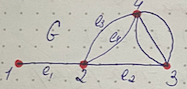
\includegraphics{image.png}
    \end{definition*}
    \item Псевдограф
    
    \begin{definition*}
      \textbf{Псевдографом} называют упорядоченную пару $(V,E)$, где $E$ - конечное мультимножество на $V^{(2)}\cup V$

      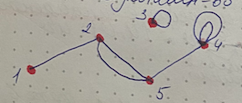
\includegraphics{pseudo.png}
    \end{definition*}
    \item Орграф(Ориентированный граф)
    
    \begin{definition*}
      $E\subseteq V\times V=\{\{u,v\}|u\in V, v\in V\}$ - \textbf{Орграф}

      $uv$ называется \textit{дугой} (вместо ребра)

      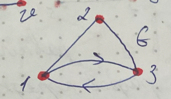
\includegraphics{Org.png}
    \end{definition*}
    \item Гиперграф
    
    \begin{definition*}
      \textbf{Гиперграфом} называют граф, где $E\subseteq2^V,2^V=\{U|U\subseteq V\}$

      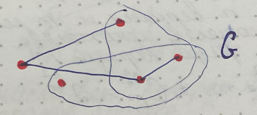
\includegraphics{Hyper.png}
    \end{definition*}
  \end{enumerate}
  \section{Помеченные графы. Изоморфизм графов}
  \begin{definition*}
    Граф назовут \textbf{помеченным}, если его вершинам принадлежат некоторые попарно различные метки.

    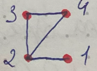
\includegraphics{metka.png}
  \end{definition*}

  Пусть $G_1, G_2$ - помеченные графы порядка n. Графы $G_1, G_2$ \textbf{равны}, если 
  $V(G_1)=V(G_2)\land E(G_1)=E(G_2)$

  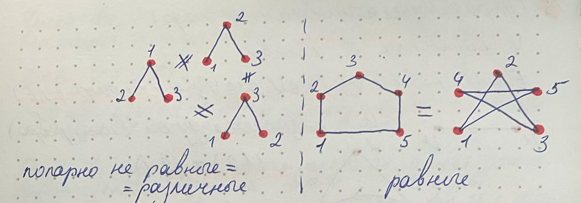
\includegraphics{eq.png}

  \begin{theorem*}
    Число всех помеченных графов порядка $n\geq1$ обозначается $l_n$ и равно $2^{C^2_n}=2^{\frac{n(n-1)}{2}}$
  \end{theorem*}
  \begin{proof}
    Пусть у графа n вершин и m рёбер. $0\leq m\leq C^2_n$. Количество подмножеств множества всех возможных рёбер графа порядка n
    $$C^0_{C^2_n}+C^1_{C^2_n}+C^2_{C^2_n}+\dots+C^{C^2_n}_{C^2_n}$$
  \end{proof}
  \begin{proof}
    ($n=5$ в качестве примера)

    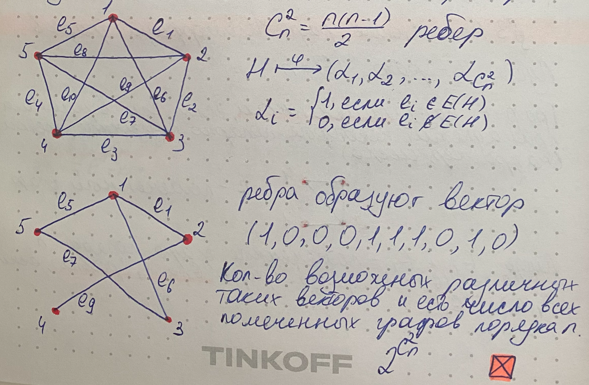
\includegraphics{proof.png}
  \end{proof}
  \subsection*{Изоморфизм графов}
  Пусть G и H - графы и $\phi:V(G)\rightarrow V(H)$  - биекция. Тогда $\phi$ - \textbf{изоморфизм} графа G на H, а G и H \textbf{изоморфны}. $G\cong H$

  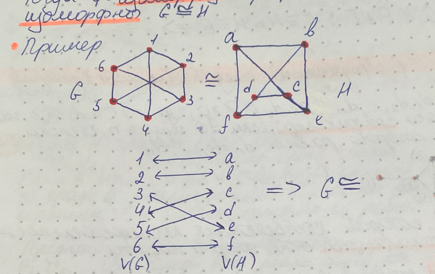
\includegraphics{example_iso.png}

  $g_n$ - число всех попарно неизоморфных графов порядка n.

  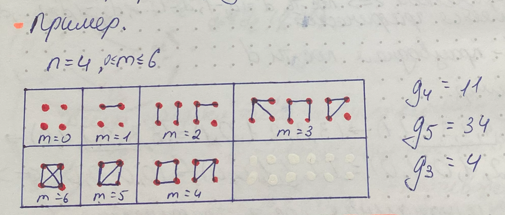
\includegraphics{ex_ni.png}

  \begin{theorem*}
    \textbf{(Лойа)}
    $$g_n\geq[\frac{2^{C^2_n}}{n!}] \text{или}g_n\sim_{n\rightarrow\infty}\frac{2^{C^2_n}}{n!}$$
  \end{theorem*}

  \textbf{Свойства} изоморфизма:
  \begin{enumerate}
    \item $G\cong G$ для конечных графов
    \item $\forall G,H:G\cong H\leftrightarrow H\cong G$
    \item $\forall G,H,F: G\cong H\cap H\cong F\rightarrow G\cong F$
  \end{enumerate}
  \section{Графические последовательности. Критерий графичности}
  \begin{definition*}
    Последовательность $d_1,d_2,\dots,d_n$, где $d_i\in Z\geq0$, где $n\geq1$
    и $d_1\geq d_2\geq\dots\geq d_n$, называется \textbf{графической}, если $\exists G$ порядка n, степени вершин которого равны $d_1,d_2,\dots,d_n$

    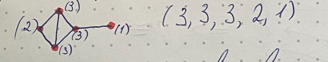
\includegraphics{graphics.png}
  \end{definition*}
  \begin{definition*}
    Граф, который соответствует последовательности называют \textbf{реализацией} этой графической последовательности.
  \end{definition*}
  \begin{theorem*}
    \textbf{(Гавела-Хакими), критерий графичности}

    Последовательность $(D=d_1,d_2,\dots,d_n)$, где $n\geq2$ и $d_1\geq d_2\geq\dots\geq d_n$, является графической \textit{тогда и только тогда, когда} последовательность $(D'=d_2-1,d_3-1,\dots,d_{d_1+1},d_{d_1+2},\dots,d_n)$ является графической.
  \end{theorem*}
  \section{Name}
  \begin{theorem*}
    Пусть $G$ -- это $(n,m)$ граф, $k$ -- число компонент связности
    Тогда
    $$n-k\leq{m}\leq\frac{(n-k)(n-k+1)}{2},.$$
  \end{theorem*}
  
  \begin{proof}
    $m\leq{n-k}$ - Доказывается по мат индукции
    
    $m\leq\frac{(n-k)(n-k+1)}{2}$ - 
    
    Берём $k\geq{2}$
    
    \begin{enumerate}
      \item рисуем $k$ полных графов
      
      \begin{tikzpicture}[main/.style = {draw, circle}]
        \node[main](1){$G_1$};
        \node[main](2)[right of=1]{$G_2$};
        \node (dots) [right of=2] {$\cdots$};
        \node[main](k)[right of=dots]{$G_k$};
      \end{tikzpicture}
      \item Вынимаем из $G_{k-1}$ точку и перемещаем её в $G_k$ (сохраняя полноту). Возьмём, что $\forall n\le k, V(G_k)\geq V(G_n)$. Тогда количество рёбер изменится на $V(G_k)-(V(G_n)-1) > 0$.
      \item Повторяем так, пока все кроме последнего подграфа не будут тривиальными (то есть пока они не будут иметь одну вершину).
      \item Самый экстремальный случай, изолированные вершины и $K_{n-k+1}$, тогда число рёбер $$C^2_{n-k+1}=\frac{(n-k)(n-k+1)}{2}.$$ 
    \end{enumerate}
  \end{proof}
  
  \begin{theorem*}
    Пусть $G$ связный граф и $e\in E(G)$.
    
    \begin{enumerate}
      \item Если $е$ принадлежит некоторому циклу, то граф $G - e$ связен
      \item Если $е$ не принадлежит никакому циклу, то граф $G - e$ содержит ровно $2$ компоненты связности
    \end{enumerate}
  \end{theorem*}
  \begin{proof}
    Возьмём $e=uv,e\in E(G)$
    
    \begin{enumerate}
      \item Если $е$ принадлежит некоторому циклу, то граф $G - e$ связен
      
      \begin{enumerate}
        \item Нарисуем цикл
        
        \begin{tikzpicture}[graph/.style = {draw, circle}, dot/.style = {draw, circle}]
          \node[dot](1){};
          \node[dot](-1)[below right of=1]{};
          \node[dot](2)[above right of=1]{};
          \node (dots) [right of=2] {$\cdots$};
          \node[dot](u)[right of=dots]{$u$};
          \node (dotsb) [right of=-1] {$\cdots$};
          \node[dot] (v) [right of=dotsb] {$v$};
          \draw (1) -- (2);
          \draw (1) -- (-1);
          \draw (-1) -- (dotsb);
          \draw (dotsb) -- (v);
          \draw (2) -- (dots);
          \draw (dots) -- (u);
          \draw (u) -- node[anchor=west]{$e$} (v) ;
        \end{tikzpicture}
        \item Удалим $e$
        
        \begin{tikzpicture}[graph/.style = {draw, circle}, dot/.style = {draw, circle}]
          \node[dot](1){};
          \node[dot](-1)[below right of=1]{};
          \node[dot](2)[above right of=1]{};
          \node (dots) [right of=2] {$\cdots$};
          \node[dot](u)[right of=dots]{$u$};
          \node (dotsb) [right of=-1] {$\cdots$};
          \node[dot] (v) [right of=dotsb] {$v$};
          \draw (1) -- (2);
          \draw (1) -- (-1);
          \draw (-1) -- (dotsb);
          \draw (dotsb) -- (v);
          \draw (2) -- (dots);
          \draw (dots) -- (u);
        \end{tikzpicture}
        
        Как можно заметить, не появилось ни одной компоненты связности.
      \end{enumerate}
      \item Если $е$ не принадлежит никакому циклу, то граф $G - e$ содержит ровно 2 компоненты связности
      \begin{enumerate}
        \item Учитывая условия выше, мы можем разделить граф на 2 части, имеющие маршрут к $u$ без $v$ и наоборот
        
        \begin{tikzpicture}[graph/.style = {draw, circle}, dot/.style = {draw, circle}]
            \node[graph](1){$G_u$};
            \node[dot](u)[right of=1]{$u$};
            \draw (1) -- (u);
            \node[dot](v)[right =0.5cm of u]{$v$};
            \draw (u) -- node[anchor=south]{$e$} (v);
            \node[graph](2)[right of=v]{$G_v$};
            \draw (v) -- (2);
        \end{tikzpicture}
        \item Удаляем ребро $e$, и видим, что появилось 2 компоненты связности
        
        \begin{tikzpicture}[graph/.style = {draw, circle}, dot/.style = {draw, circle}]
            \node[graph](1){$G_u$};
            \node[dot](u)[right of=1]{$u$};
            \draw (1) -- (u);
            \node[dot](v)[right =0.5cm of u]{$v$};
            \node[graph](2)[right of=v]{$G_v$};
            \draw (v) -- (2);
        \end{tikzpicture}
      \end{enumerate}
    \end{enumerate}
  \end{proof}
  
  \section{Метрические характеристики графов}
  Для параграфа: G - связен

  \textbf{Определение.} Расстояние $d(u,v)$ между вершинами $u\neq v$ графа G --  \textit{длинна кратчайшей простой цепи}, если $u=v$, то $d(u,v)=0$
  
  \textbf{Свойства:}
  \begin{enumerate}
    \item \textbf{Свойство неотрицательности.}
    $$d(u,v)\geq 0\ \text{и}\ d(u,v) = 0 \Leftrightarrow u=v,\ \forall u,v\in V(G).$$
    \item \textbf{Свойство симметрии.} 
    $$d(u,v)=d(v,u),\ \forall u,v\in V(G).$$ 
    \item \textbf{Свойство треугольников.}
    $$d(u,v)\leq d(u,w)+d(w,u),\ \forall u,v\in V(G).$$
  \end{enumerate}
  
  \textbf{Определение.} \textit{Эксцентриситетом вершины} называется величина $$e(v)=\max d(v,u),v\in V(G),$$ то есть максимальное расстояние от вершины до другой какой-либо вершины графа).
  
  \textbf{Определение.} \textit{Радиусом графа} называется величина $$r(G)=\min e(v),\ v\in V(G).$$
  
  \textbf{Определение.} \textit{Диаметром графа} называется величина $$d(G)=\max e(v),\ v\in V(G).$$
  
  \textbf{Определение.} \textit{Вершина в графа $G$ называется \textit{центральной}, если $e(v)=r(G)$ и \textbf{периферической}, если $e(v)=d(G)$.}
  
  \textbf{Определение.} Центр графа, множество всех его центральных вершин, перефирия, перефирийных.
  
  Пример, в круге Эксцентриситет вершины:

  \begin{tikzpicture}[graph/.style = {draw, circle}, dot/.style = {draw, circle}]
    \node[dot](1){4};
    \node[dot](2)[above right of=1]{3};
    \node[dot](3)[right of=2]{2};
    \node[dot](4)[right of=3]{3};
    \node[dot](5)[below right of=4]{4};
    \draw (1) -- (2) -- (3) -- (4) -- (5);
  \end{tikzpicture}
  $r(P_5)=2, d(P_5)=4$
  
  \begin{theorem*}
    Для любого графа $H$ существует граф $G$, центр которого порождает $H$.
  \end{theorem*}
  \begin{proof}
    \begin{enumerate}
        \item Возьмём граф $H$
        
        \begin{tikzpicture}[graph/.style = {draw, circle}, dot/.style = {draw, circle}]
            \node[graph](H){$H$};
        \end{tikzpicture}
        \item Добавим к нему вершины $x,y,z,t$, $x$ и $y$ Соедениены со всеми вершинами $H$
        
        \begin{tikzpicture}[graph/.style = {draw, circle}, dot/.style = {draw, circle}]
            \node[graph](H){$H$};
            \node[dot](x)[left =0.5cm of H]{$x$};
            \node[dot](y)[right =0.5cm of H]{$y$};
            \node[dot](z)[below of=x]{$z$};
            \node[dot](t)[below of=y]{$t$};
            \draw (z) -- (x) (y) -- (t);
            \draw[double] (x) -- (H) -- (y);
        \end{tikzpicture}

        Как видно $\forall v \in V(H), e(v)=r(G)=2$
    \end{enumerate}
  \end{proof}
  \begin{theorem*}
  Для любого связного графа ж верно: $r(G)\leq d(G)\leq 2r(G)$
  \end{theorem*}
  \begin{proof}
    .
    \begin{enumerate}
        \item $r(G)\leq d(G)$ - очевидно
        \item $diam(G)\leq 2r(G)$. Берём две переферичиские$(u,v)$ и одну центральную$(w)$. Тогда данное равенство получается через равенство треугольника:
        
        \begin{tikzpicture}[graph/.style = {draw, circle}, dot/.style = {draw, circle}]
            \node[dot](w){$w$};
            \node[dot](u)[below left of=w]{$u$};
            \node[dot](v)[below right of=w]{$v$};
            \draw (u) -- (w) -- (v);
            \draw[dotted] (u) -- (v);
        \end{tikzpicture}

        По свойству треугольников:$$d(u,v)\leq d(u,w)+d(w,v)\rightarrow d(G)\leq2r(G)$$
    \end{enumerate}
  \end{proof}
\end{document}
